


%%%%%%%%%%%%%%%%%%%%%%%%%%%%%%%%%%%%%%%%%%%%%%%%%%%%%%%%%%%%%%%%%%%%%%%%
%%%%%% Definitionen
%%%%%%%%%%%%%%%%%%%%%%%%%%%%%%%%%%%%%%%%%%%%%%%%%%%%%%%%%%%%%%%%%%%%%%%%

\section{Mathematische Definitionen}
Zu Beginn definieren wir die grundlegenden mathematischen Begriffe. Als wichtigste Grundlage dient 
hierbei das Konstrukt des \red{ungerichteten} Graphen.
\begin{definition}[Graph] ~\\
Ein (ungerichteter) \textbf{Graph} $G = (V,E)$ ist ein Tupel bestehend aus einer Knotenmenge $V$ und einer Kantenmenge
 $E$. Eine Kante verbindet zwei Knoten miteinander und ist damit eine Menge, aus zwei Knoten.
 Es gilt: $E \subseteq \{ \{u,v\} |\ u,v \in V, u \neq v \}$.  
\end{definition}
\red{In dieser Arbeit} spielt eine spezielle Klasse von Graphen, bipartite Graphen, eine zentrale Rolle.
Bei einem bipartiten Graphen kann man die Knoten in zwei Mengen teilen, sodass alle Kanten nur zwischen den 
beiden Mengen verlaufen und nicht innerhalb einer Menge. Formal bedeutet dies:
\begin{definition}[bipartiter Graph] ~\\
Ein Graph $G=(V,E)$ heißt \textbf{bipartit}, wenn es Teilmengen $V_1 \subset V$ und $V_2 \subset V$ gibt, für die 
$V_1 \cup V_2 = V$ und $V_1 \cap V_2 = \emptyset$ gilt,
 sodass für jede Kante $e \in E$ ein $u \in V_1$ und ein $v \in V_2$ existiert, sodass $e = \{u,v\}$ gilt.
Die Knotenmengen $V_1$ und $V_2$ werden auch als Partitionen bezeichnet.
\end{definition}

\noindent
Ein Beispiel für einen bipartiten Graphen sieht man in Abbildung \ref{fig:beispiel_bipartit}. Dabei gilt für die Partitionen:
$V_1 = \{v_1,v_2,v_3,v_4\}$ und $V_2 = \{v_5,v_6,v_7,v_8\}$. Man sieht deutlich, dass alle Kanten die Partitionen
$V_1$ und $V_2$ ''kreuzen''.

\begin{figure}[h]
%bipartiter graph
\centering
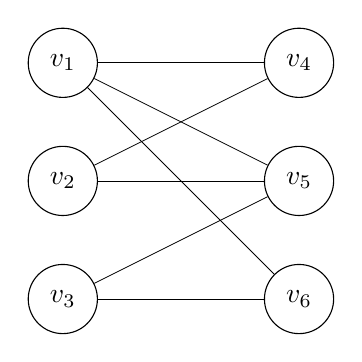
\begin{tikzpicture}
\tikzset{node style/.style={shape=circle,draw=black, inner sep=5pt,}}
                                
\node[node style] at (0, 0)     (1)     {$v_1$};
\node[node style] at (0, -1.5)   (2)     {$v_2$};
\node[node style] at (0, -3)     (3)     {$v_3$};
%\node[node style] at (0, -4.5)   (4)     {$v_4$};

\node[node style] at (3, 0)     (5)     {$v_4$};
\node[node style] at (3, -1.5)   (6)     {$v_5$};
\node[node style] at (3, -3)   (7)     {$v_6$};
%\node[node style] at (3, -4.5)   (8)     {$v_8$};

   
\draw[line width=0.1mm, >=latex]
            (1)     edge[right]    node {} (5)
            (1)     edge[right]    node {} (6)
            (1)     edge[right]    node {} (7)
            (2)     edge[right]    node {} (5)
            (2)     edge[right]    node {} (6)
            (3)     edge[right]    node {} (6)
            %(4)     edge[right]    node {} (5)
            %(4)     edge[right]    node {} (8)
            (3)     edge[right]    node {} (7)
;
\end{tikzpicture}
\caption{Beispiel eines bipartiten Graphen}
\label{fig:beispiel_bipartit}
\end{figure}
\red{überleitung}
Für einen \ct ist vor allem der Begriff der Nachbarschaft, genauer der gemeinsamen und disjunkten 
Nachbarschaft, entscheidend.
\begin{definition}[Nachbarschaft]~\\
Ein Knoten $u \in V$ heißt \textbf{benachbart} (oder \fett{adjazent}) zu einem 
anderen Knoten $v \in V$, wenn es eine Kante $\{u,v\} \in E $ gibt. Die Menge $N(u)$ aller adjazenten Knoten
von $u$ nennt man \fett{Nachbarschaft}.
\end{definition}
\begin{definition}[gemeinsame und disjunkte Nachbarschaft]~\\
	Die \fett{gemeinsame} Nachbarschaft $N_{c}(u,v)$ zweier Knoten $u$ und $v$ ist die Menge aller Knoten, die sowohl
	zu $u$ als auch zu $v$ adjazent sind. In der \fett{disjunkten} Nachbarschaft $N_{d}(u,v)$ von $u$ und $v$ sind dagegen 
	alle Knoten die nur zu einem der beiden Knoten adjazent sind. \\
	Es gilt also $N_{c}(u,v) = N(u) \cap N(v)$ und $N_{d}(u,v) = \big(N(u) \cup N(v)\big)\setminus \big(N(u) \cap N(v) \big)$
\end{definition}

\red{Dabei bemerken wir, dass in einem bipartiten Graphen zwei Knoten aus einer Partitionsklasse nie
in der gegenseitigen Nachbarschaft liegen können. Dieser Fakt wird beim Bipartiten \gc ausgenutzt.
}
\blue{Zuletzt} sind noch die Begriffe Knotengrad und Gradsequenz relevant.
\begin{definition}[Knotengrad]~\\
Der \fett{Grad} eines Knotens $v \in V$ wird mit $\deg(v)$ bezeichnet und entspricht die Anzahl
der adjazenten Knoten von $v$. Es gilt also $\deg(v) = |N(v)|$ für alle Knoten $v\in V$.
\end{definition}
\begin{definition}[Gradsequenz]~\\
Die \fett{Gradsequenz} eines Graphen $G = (V,E)$ mit $|V| = n$ Knoten ist gegeben durch das Tupel
$D = (d_{1}, \dots, d_{n})$, wobei $d_{i} = \deg(v_{i})$ der Grad des Knotens $v_{i}$ ist.
\end{definition}
\noindent
Im bipartiten Graph aus Abbildung \ref{fig:beispiel_bipartit} hat beispielsweise
der Knoten $v_{1}$ dem Grad $\deg(v_{1}) = 3$. Für die Gradsequenz des Graphen gilt: 
$D = (3,2,2,2,3,2)$. \red{kann man das so lassen?}




%%%%%%%%%%%%%%%%%%%%%%%%%%%%%%%%%%%%%%%%%%%%%%%%%%%%%%%%%%%%%%%%%%%%%%%%
%%%%%% NetworKit
%%%%%%%%%%%%%%%%%%%%%%%%%%%%%%%%%%%%%%%%%%%%%%%%%%%%%%%%%%%%%%%%%%%%%%%%
\section{\nk}

\nk \cite{nk} ist ein Open-Source Projekt, dass es zum Ziel hat, ''Werkzeuge für die
Analyse großer Netzwerke, in den Größenordnungen von Tausenden bis Milliarden 
von Kanten, zur Verfügung zu stellen''.
\footnote{aus \cite{nk} abgerufen am 10.2.2020}
\\
Innerhalb von \nk Gibt es einfache Graph Datenstrukturen \red{blabla}
\\
Man kann es mit python nutzen \red{blabla}
\blue{hmmm keine Ahnung}




%%%%%%%%%%%%%%%%%%%%%%%%%%%%%%%%%%%%%%%%%%%%%%%%%%%%%%%%%%%%%%%%%%%%%%%%
%%%%%% Datenstruktur
%%%%%%%%%%%%%%%%%%%%%%%%%%%%%%%%%%%%%%%%%%%%%%%%%%%%%%%%%%%%%%%%%%%%%%%%

\section{Datenstruktur}
In \nk \red{\cite{nk} muss das immer hin, wenn \nk erwähnt wird?!} werden Graphen in einer eigenen Datenstruktur gespeichert. Um den Algorithmus 
zu vereinfachen, wird der Graph in eine einfachere Datenstruktur transformiert.
Diese Datenstruktur muss so aufgebaut sein, dass man damit effizient zwei zufällige
Knoten auswählen, die (disjunkten und gemeinsamen) Nachbarschaften berechnen und Knoten aus der
disjunkten Nachbarschaft tauschen kann. Dafür eignet sich am Besten  
eine Art Adjazenzlistendarstellung des Graphen, wobei jedoch keine echten verketteten
Listen verwendet werden, sondern lediglich Vektoren. 
Es wird also für einen Knoten
$v \in V$ ein Vektor erstellt, indem alle adjazenten Knoten gespeichert sind.
Da wir ausschließlich bipartite Graphen betrachten werden, speichern wir noch in 
einem weiteren Vektor die Knoten von einer der beiden Bipartitionsklassen \red{die größere? oder egal? }. Diesen
werden wir als \red{\fett{\partvek}} bezeichnen.
\\
Die Vektoren sind dabei vom \cpp \red{Datentyp   (falsches wort/was ist richtig? container?)} \texttt{std::vector}.
\red{Dieser Container unterstützt random access in $\O(1)$}

\red{KNOTEN ENTSPRECHEN INTS!?}
%%%%%%%%%%%%%%%%%%%%%%%%%%%%%%%%%%%%%%%%%%%%%%%%%%%%%%%%%%%%%%%%%%%%%%%%
%%%%%% Global Curveball
%%%%%%%%%%%%%%%%%%%%%%%%%%%%%%%%%%%%%%%%%%%%%%%%%%%%%%%%%%%%%%%%%%%%%%%%

\section{Global Curveball \red{(auf bipartiten Graphen)}}
Wie \red{in der Einleitung beschrieben}, ist \gc ein Verfahren zum Randomisieren von Graphen.
Dabei ist als Eingabe ein beliebiger bipartiter Graph gegeben, der in einen \red{anderen/zufälligen}
Graph mit äquivalenter Gradsequenz transformiert werden soll.
\\
Die Aufgabe ist also, bei einer gegebenen Gradsequenz $D$, eine uniform verteilte \red{Stichprobe???}
aus der Menge aller Graphen mit Gradsequenz $D$ zurückzugeben. Durch das Ausführen von \gc 
bleibt also für jeden Knoten $v\in V$ sein Grad $\deg(v)$ erhalten. \red{(aus survey übernommen)}
\\
\\
\red{\Large
Ein allgemeiner Ansatz wäre...
Um dies zu erreichen kann man Kanten Tauschen....
Was soll da dazu??}
\\
\\
\\
\fett{\cb} ist \red{nun} ein Prozess, der ähnlich zum Kanten Tauschen ist. Bei einem \ct werden
zwei verschiedene Knoten $u$ und $v$ ($u\neq v$) zufällig uniform verteilt ausgewählt, deren Nachbarschaft
zufällig \red{durchmischt (oder lieber shuffle?)} wird. Da bei der \red{bipartiten Version}  von \cb{}
die Knoten $u$ und $v$ beide aus der gleichen Partitionsklasse gezogen werden, ist sichergestellt, dass
es keine Kante zwischen $u$ und $v$ gibt. \red{Somit sind die beiden Knoten nicht in der jeweils anderen Nachbarschaft
enthalten, es gilt folglich $u\notin N(v)$ und $v\notin N(u)$}.
Wird die komplette Nachbarschaft $N(u) \cup N(v)$ durchmischt könnte es \red{passieren}, 
dass dadurch \red{Multikanten} (mehrere Kanten zwischen zwei Knoten) entstehen,  
nämlich genau dann, wenn ein Knoten aus der gemeinsamen Nachbarschaft getauscht wird, sodass er dann in 
einer der Nachbarschaften doppelt vorkommt.
Um dies zu Vermeiden werden ausschließlich die Knoten aus der disjunkten Nachbarschaft $N_{d}(u,v)$ getauscht.
Ein Beispiel für solch einen Tausch ist in Abbildung \ref{fig:curveball_trade_graph} gegeben.
%
%
%
%%%%% CURVEBALL TRADE auf graph
\begin{figure}[h]
\centering
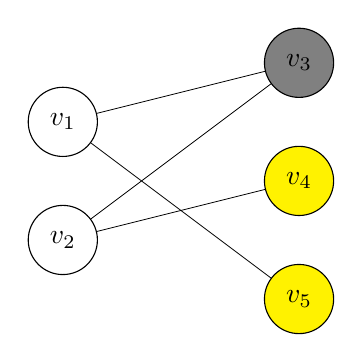
\begin{tikzpicture}
		\tikzset{node style/.style={shape=circle,draw=black, inner sep=5pt,}}
                                
\node[node style] at (0, -0.75)     (1)     {$v_1$};
\node[node style] at (0, -2.25)   (2)     {$v_2$};


\node[node style, fill=gray] at (3, 0)     (5)     {$v_3$};
\node[node style, fill=yellow] at (3, -1.5)   (6)     {$v_4$};
\node[node style, fill=yellow] at (3, -3)   (7)     {$v_5$};


   
\draw[line width=0.1mm, >=latex]
            (1)     edge[right]    node {} (5)
            (1)     edge[right]    node {} (7)
            (2)     edge[right]    node {} (5)
            (2)     edge[right]    node {} (6)

;
\end{tikzpicture}
\hspace{2cm}
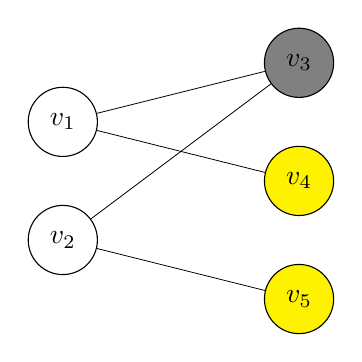
\begin{tikzpicture}
\tikzset{node style/.style={shape=circle,draw=black, inner sep=5pt,}}
                                
\node[node style] at (0, -0.75)     (1)     {$v_1$};
\node[node style] at (0, -2.25)   (2)     {$v_2$};

\node[node style, fill=gray] at (3, 0)     (5)     {$v_3$};
\node[node style, fill=yellow] at (3, -1.5)   (6)     {$v_4$};
\node[node style, fill=yellow] at (3, -3)   (7)     {$v_5$};


\draw[line width=0.1mm, >=latex]
            (1)     edge[right]    node {} (5)
            (1)     edge[right]    node {} (6)
            (2)     edge[right]    node {} (5)
            (2)     edge[right]    node {} (7)

;
\end{tikzpicture}
\caption{Beispiel eines Curveball-Tausches}
\label{fig:curveball_trade_graph}
	
\end{figure}
%
%
%
%
%
Dabei wird der \ct auf den Knoten $v_{1}$ und $v_{2}$ ausgeführt. 
Für die \red{(grau markierte)} gemeinsame Nachbarschaft gilt $N_{c}(v_{1},v_{2}) = \{v_{3}\}$, 
die disjunkte Nachbarschaft $N_{d}(v_{1},v_{2}) = \{v_{4},v_{5}\}$ ist in gelber Farbe gekennzeichnet.
In diesem Beispiel gibt es nur die zwei gegeben Graphen, die durch Tauschen der disjunkten 
Nachbarschaft entstehen können. \red{Ein \ct würde dann jeweils mit Wahrscheinlichkeit 0.5 einen der beiden 
Graphen zurückgeben.}
%
%
%
%
%
%%%%% CURVEBALL TRADE auf Vektor
\begin{figure}[h]
\centering
  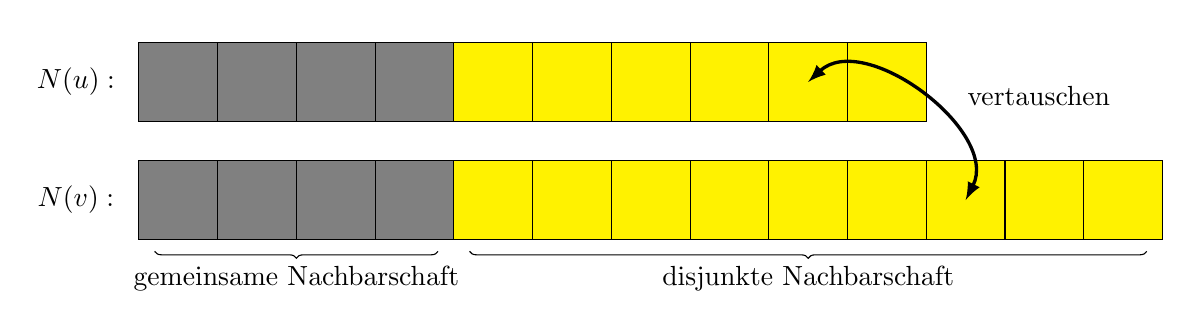
\begin{tikzpicture}[decoration=brace]
      
      
    %% COMMON FÄRBEN  
    \foreach \x in {0,1,2,3}
		{
			\fill [ fill =gray, draw =black ]  (\x ,0) rectangle (\x+1 ,1) ;
			\fill [ fill =gray, draw =black ]  (\x ,-1.5) rectangle (\x+1 ,-0.5) ;
		};

    %% DISJOINT OBEN FÄRBEN  
    \foreach \x in {4,5,6,7,8,9}
		{
			\fill [ fill =yellow, draw =black ]  (\x ,0) rectangle (\x+1 ,1) ;
		};
		
	%% DISJOINT UNTEN FÄRBEN  
    \foreach \x in {4,5,6,7,8,9,10,11,12}
		{
			\fill [ fill =yellow, draw =black ]  (\x ,-1.5) rectangle (\x+1 ,-0.5) ;
		};
    
\node[] at (-0.8, 0.5)     (5)     {$N(u):$};
\node[] at (-0.8, -1)     (5)     {$N(v):$};
    
    % untere geschweifte Klammer mit Text darunter:
    \draw[decorate, yshift=-1ex] (3.8,-1.5) -- node[below=0.4ex] {gemeinsame Nachbarschaft} (0.2,-1.5);
    \draw[decorate, yshift=-1ex] (12.8,-1.5) -- node[below=0.4ex] {disjunkte Nachbarschaft} (4.2,-1.5);


	\draw[bend left=80, <->,>=latex, very thick] (8.5,0.5) to  node[right= 3ex] {vertauschen} (10.5,-1) ;

  \end{tikzpicture}
  \caption{\ct auf den Vektoren}
  \label{fig:curveball_trade_vector}
  
\end{figure}
%
%
%
%
In Abbildung \ref{fig:curveball_trade_vector} ist eine \red{Skizze} gegeben, wie man sich einen
\ct in der Datenstruktur, also den Vektoren vorstellen kann. Dabei werden zuerst die Elemente
der beiden Vektoren in gemeinsame und disjunkte Nachbarschaft aufgeteilt. Die gemeinsame Nachbarschaft ist
wieder in grau gekennzeichnet, die disjunkte in gelb. Bei einem \ct bleiben dann die Elemente 
der gemeinsame Nachbarschaft unverändert, während die Elemente aus der disjunkten Nachbarschaft zufällig zwischen den beiden 
Vektoren getauscht werden.
\\
Ein \fett{Globaler \ct} besteht aus mehreren Curveball-Tauschen, wobei möglichst jeder Knoten aus der \red{Partition}
Teil eines Curveball-Tausches sein soll.
%
%
% 
\begin{figure}[h]
\centering
  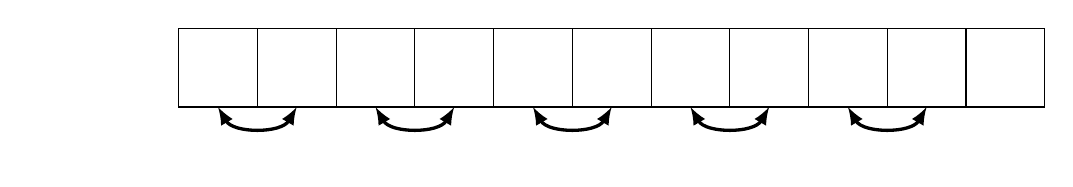
\begin{tikzpicture}[decoration=brace]
      
      
    %% COMMON FÄRBEN  
    \foreach \x in {0,1,2,3,4,5,6,7,8,9,10}
		{
			\fill [ fill =white, draw =black ]  (\x ,0) rectangle (\x+1 ,1) ;
		};
    
\node[] at (-1.8, 0.5)     (5)     {\partvek};
    
    % untere geschweifte Klammer mit Text darunter:
    \foreach \x in {0,2,4,6,8}
		\draw[bend angle=60,bend right,  <->,>=latex, very thick] (\x+0.5,0) to  node[below= 1ex] {\cb} (\x+1.5,0) ;

  \end{tikzpicture}
  \caption{\gc auf dem Partitions Vektor}
  \label{fig:global_curveball_trade_vector}
  
\end{figure}
%
%
%
In Abbildung \ref{fig:global_curveball_trade_vector} ist eine Skizze des Partitionsvektors gegeben.
Für einen \gc Tausch wird dieser Vektor zuerst \red{geshuffelt (zufällig permutiert)}, sodass jedes Element an einer zufälligen
Position steht. Dann wird jeweils parallel ein \ct auf den Elementen eins und zwei, drei und vier, usw. ausgeführt.
Durch das zufällige Permutieren des Vektors zu Beginn, wird also jeder der Curveball-Tausche auf zwei zufälligen
Knoten ausgeführt. Hat der \partvek eine ungerade Anzahl an Elementen, bleibt am Ende ein Element übrig, 
welches nicht Teil von einem \ct ist. Bei der Parallelisierung an dieser Stelle, wird ausgenutzt, dass 
der zugrundeliegende Graph bipartit ist. Da es innerhalb der Partition keine zwei Knoten gibt, welche  
durch eine Kante miteinander verbunden sind, wird bei einem \ct auf beliebigen Knoten $u$ und $v$ 
die Nachbarschaft eines anderen Knotens $x$  aus der gleichen Partition nicht geändert. Somit
\red{''überschneiden'' sich} die verschiedenen Curveball-Tausche nicht, man kann sie also \red{gleichzeitig
laufen lassen}. 
\\
\\
Im vollständigen Randomisierungs-Algorithmus werden schließlich mehrere solcher \gc Tausche nacheinander
durchgeführt.\red{Wie viele?!}



~\\
\\
\\
\red{Man KONVERGIERT zu einem uniform sample...?}










%%%%%%%%%%%%%%%%%%%%%%%%%%%%%%%%%%%%%%%%%%%%%%%%%%%%%%%%%%%%%%%%%%%%%%%%
%%%%%% Parallelität
%%%%%%%%%%%%%%%%%%%%%%%%%%%%%%%%%%%%%%%%%%%%%%%%%%%%%%%%%%%%%%%%%%%%%%%%

\section{Parallelisierung}

\red{muss hier noch was dazu?!}
